\documentclass[tikz,border=7pt]{standalone}
\usepackage{amsmath}
\usetikzlibrary{arrows.meta,positioning,fit}

\tikzset{
  comp/.style={draw,rectangle,minimum width=28mm,minimum height=12mm,align=center},
  signal/.style={-{Latex[length=2.2mm]},thick},
  area/.style={draw,dashed,rounded corners=3pt,inner sep=7mm}
}

\begin{document}
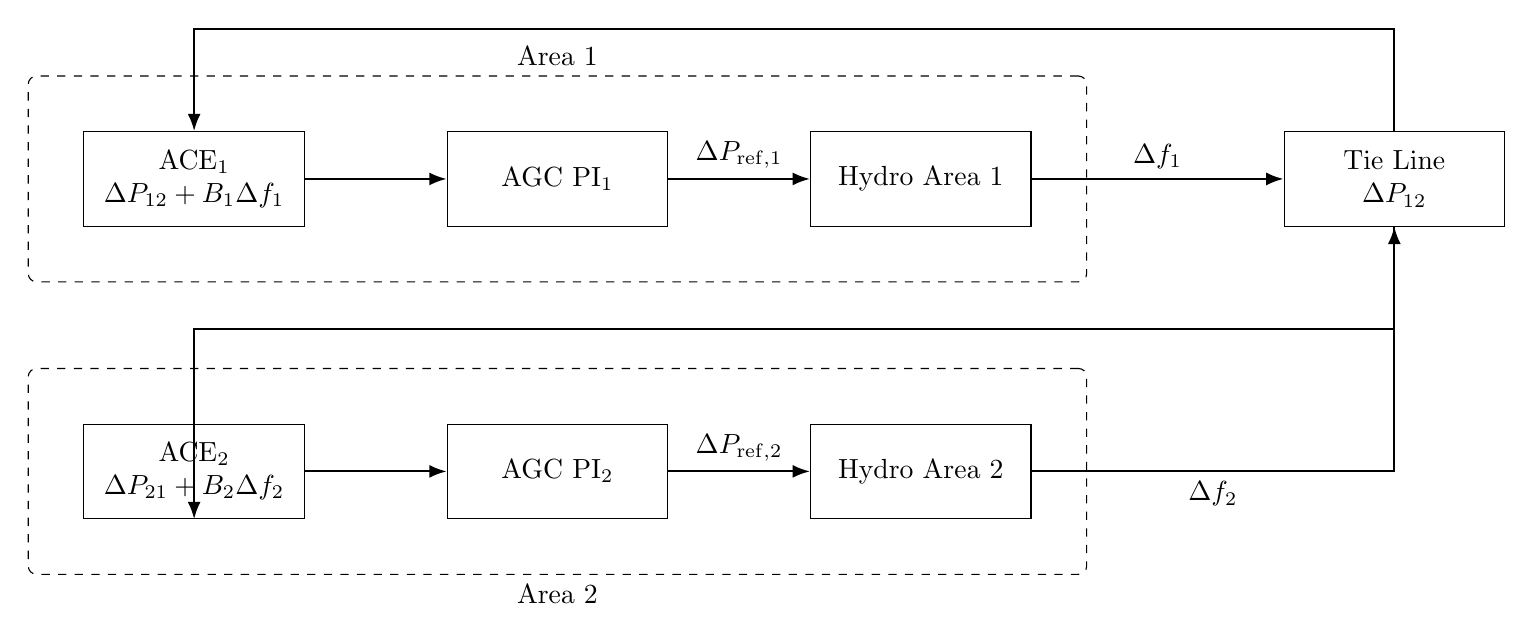
\begin{tikzpicture}[node distance=12mm and 18mm]

\node[comp] (ace1) {ACE$_1$\\$\Delta P_{12}+B_1\Delta f_1$};
\node[comp,right=of ace1] (agc1) {AGC PI$_1$};
\node[comp,right=of agc1] (plant1) {Hydro Area 1};

\node[comp,below=25mm of ace1] (ace2) {ACE$_2$\\$\Delta P_{21}+B_2\Delta f_2$};
\node[comp,right=of ace2] (agc2) {AGC PI$_2$};
\node[comp,right=of agc2] (plant2) {Hydro Area 2};

\node[comp,right=32mm of plant1] (tie) {Tie Line\\$\Delta P_{12}$};

\draw[signal] (ace1) -- (agc1);
\draw[signal] (agc1) -- node[above] {$\Delta P_{\mathrm{ref},1}$} (plant1);
\draw[signal] (ace2) -- (agc2);
\draw[signal] (agc2) -- node[above] {$\Delta P_{\mathrm{ref},2}$} (plant2);

\draw[signal] (plant1) -- node[above] {$\Delta f_1$} (tie);
\draw[signal] (plant2.east) -| node[pos=0.25,below] {$\Delta f_2$} (tie.south);

\draw[signal] (tie.north) |- ++(0,13mm) -| (ace1.north);
\draw[signal] (tie.south) |- ++(0,-13mm) -| (ace2.south);

\node[area,fit=(ace1)(agc1)(plant1),label=above:{Area 1}] {};
\node[area,fit=(ace2)(agc2)(plant2),label=below:{Area 2}] {};

\end{tikzpicture}
\end{document}
